\section{HI bias parameters} \label{app1}

We follow \cite{Umeh:2015gza} to compute $b_{1}$ and $b_{2}$ from a halo-model approach:
\begin{align}
b_{1} &= 1 + \left\langle \frac{2p+\big(q\nu - 1\big)\big[1+(q\nu)^{p}\big]}{\delta_{\rm cr}\big[1+(q\nu)^{p}\big]} \right\rangle _{\!\!\!\rm m}  \!\!, \label{e1.16} \\
b_{2} &= \frac{8}{21}\big(b_{1}-1\big) + \left \langle \frac{2p\big(2p+2\nu q-1\big)+ q\nu\big(q\nu-3\big)\big[1+(q\nu)^{p}\big]}{\delta_{\rm cr}^{2}\big[1+(q\nu)^{p}\big]}  \right \rangle _{\!\!\!\rm m}  \!\!, \label{e1.17}
\end{align}
where the parameters $p$, $q$ and $\nu$ are related to the Sheth-Tormen distribution function (see \cite{Sheth:1999su, Sheth:2001dp, Sheth:1999mn} for more details), and $\delta_{\rm cr}$ is the critical density at which halos collapse spherically \cite{Kitayama:1996ne}, 
\begin{equation}
\delta_{\rm c}(z) = \frac{3(12\pi)^{2/3}}{20}\big[1+0.0123\log{\Omega_{\rm m} (z)}\big] \,. \label{e1.20}
\end{equation}
The mass average is defined by 
\begin{equation}
\big\langle X_{h}(z,\bm{x}) \big\rangle _{\rm m}  = \frac{\int_{M_{-}}^{M_{+}} \ud M\,X_{h}(z,\bm{x},M)\,M_{\mathrm{HI}}(M)\,n_{h}(z,\bm{x},M)}{\int_{M_{-}}^{M_{+}} \ud M\,M_{\mathrm{HI}}(M)\,n_{h}(z,\bm{x},M)} \, , \label{e1.18}
\end{equation}
where $M$ is the mass of {halos} that can host HI gas, and $M_{\pm}$ are the lower and upper mass limits, which are  related to the circular velocities  of the galaxies \citep{Bull:2014rha}. $n_{h}$ is the halo mass function \citep{Sheth:1999su, Sheth:2001dp,Tellarini:2015faa}, and $M_{\rm HI}$ is the HI mass function, which is assumed to follow a power law  \citep{Santos:2015gra},
\begin{equation}
M_{\mathrm{HI}}(M) \propto M^{0.6} \,. \label{e1.19}
\end{equation}
 Figure~\ref{fig1} shows the numerical results from \eqref{e1.16} and \eqref{e1.17}. Fitting formulas for the bias parameters are
\bea
b_{1}(z)& = & 0.754 + 0.0877z + 0.0607z^{2} - 0.00274z^{3}\,, \label{e1.27} \\
b_{2}(z) &= & -0.308 - 0.0724z - 0.0534z^{2} + 0.0247z^{3}\,. \label{e1.28}
\eea
Assuming that  halo formation is a local process in Lagrangian space and that there is no initial tidal bias, the tidal bias is \cite{Tellarini:2015faa}:
\begin{equation}
b_{s^{2}} = \frac{4}{7}\big(1-b_{1}\big)\,.\label{e1.21} 
\end{equation} 

\clearpage

\section{MeerKAT and SKA system temperatures} \label{app2}
\vspace*{-0.5cm}
\begin{table}[! ht]
\centering
\caption{\label{tab5} System temperatures for MeerKAT and SKA1-MID, used in Figure~\ref{fig2} (from \cite{Fonseca:2019qek}).} 
\vspace*{0.2cm}
  \begin{tabular}{|l|l|l|l|l|l|l|l|}
    \hline
      \multicolumn{2}{|c|}{MeerKAT L Band} &
      \multicolumn{2}{c|}{MeerKAT UHF Band} &
      \multicolumn{2}{c|}{SKA1-MID Band 1} & 
      \multicolumn{2}{c|}{SKA1-MID Band 2} \\
      \hline \hline
    $~~~~z~~$ & $~~T_{\rm sys}\;/\;\rm K~~~$ & $~~~z~$ & $~~~~T_{\rm sys}\;/\;\rm K~~$ & $~~~z~$ & $~~T_{\rm sys}\;/\;\rm K~~$ & $~~~~z~~$ & $~~T_{\rm sys}\;/\;\rm K~~$ \\
    \hline
    
  %& & & & & & & \\
  
     0.136 & ~~~~19.2 & 0.420 & ~~~~~~20.3 & 0.403 & ~~~~27.2 & 0.115 & ~~~~16.4 \\
    
     0.183 & ~~~~19.7 & 0.495 & ~~~~~~21.0 & 0.470 & ~~~~26.9 & 0.168 & ~~~~16.6 \\
    
     0.235 & ~~~~20.3 & 0.578 & ~~~~~~21.7 & 0.539 & ~~~~26.8 & 0.223 & ~~~~16.8 \\
    
     0.291 & ~~~~20.9 & 0.671 & ~~~~~~22.5 & 0.612 & ~~~~26.9 & 0.280 & ~~~~17.0 \\
    
     0.352 & ~~~~21.5 & 0.775 & ~~~~~~23.5 & 0.767 & ~~~~27.5 & 0.341 & ~~~~17.2 \\
    
    0.420 & ~~~~22.3 & 0.893 & ~~~~~~24.7  & 0.850 & ~~~~28.1 & 0.403 & ~~~~17.6 \\
    
    0.495 & ~~~~23.1 & 1.03 & ~~~~~~26.1   & 0.938 & ~~~~28.8 & 0.470  & ~~~~18.0 \\
    
    0.578 & ~~~~24.0 & 1.18 & ~~~~~~27.9   & 1.03  & ~~~~29.8 &        &  \\
    
          &          & 1.37 & ~~~~~~30.3   & 1.12  & ~~~~30.8 &        &  \\
     
          &          & 1.45 & ~~~~~~31.5   & 1.22  & ~~~~32.1 &        &  \\
    
          &          &      &              & 1.33  & ~~~~33.5 &        &   \\
    
          &          &      &              & 1.44  & ~~~~35.2 &        &    \\
    
          &          &      &              & 1.55  & ~~~~37.1 &        &   \\
    
          &          &      &              & 1.67  & ~~~~39.2 &        &   \\
    
          &          &      &              & 1.80  & ~~~~41.6 &        & \\
    
          &          &      &              & 1.93  & ~~~~44.2 &        &  \\
    
          &          &      &              & 2.07  & ~~~~47.2 &        &  \\
    
          &          &      &              & 2.22  & ~~~~50.6 &        &  \\
    
          &          &      &              & 2.37  & ~~~~54.4 &        &  \\
    
          &          &      &              & 2.54  & ~~~~58.6 &        &  \\
    
          &          &      &              & 2.69  & ~~~~63.4 &        &  \\
    
          &          &      &              & 2.87  & ~~~~68.8 &        &  \\
    
          &          &      &              & 3.05  & ~~~~74.8 &        &  \\
    
 %         &          &      &              &       &          &        &  \\
    \hline
  \end{tabular}
\end{table}
\vspace*{-0.5cm}
 \begin{figure}[! h]
\centering
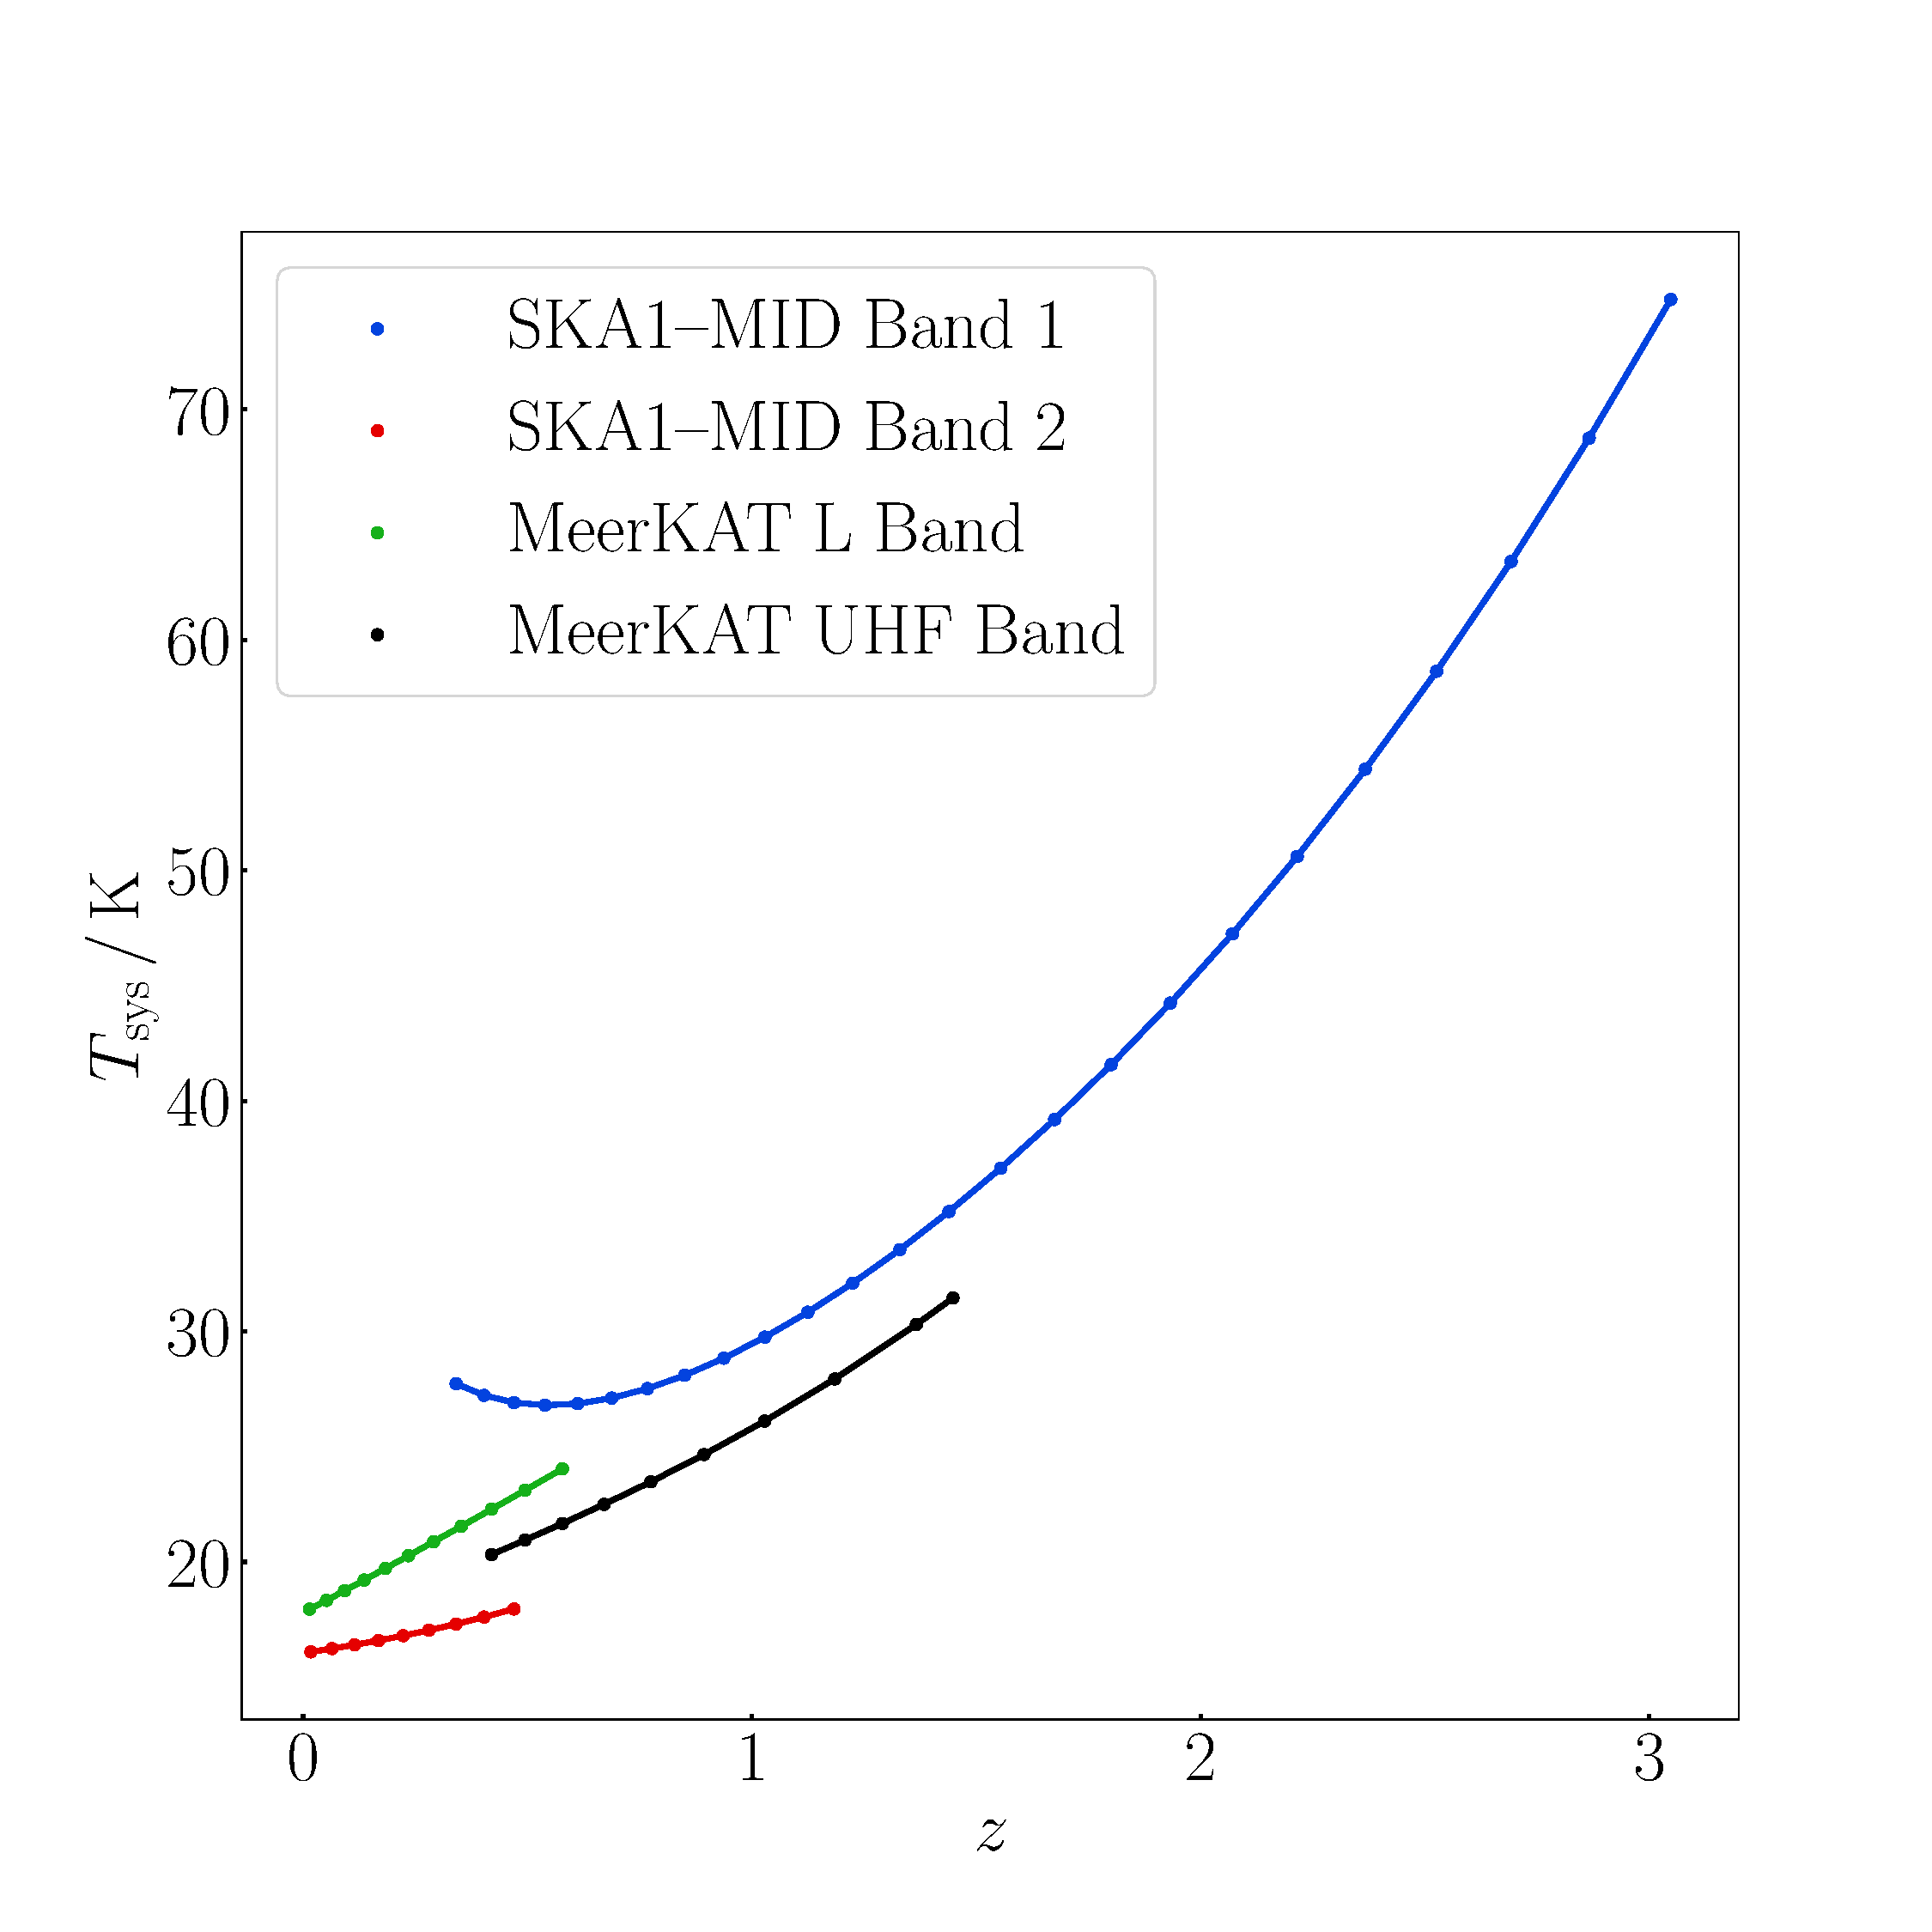
\includegraphics[width=.49\textwidth]{tSys}
\vspace*{-0.5cm}
\caption{$T_{\rm sys}$ for the different frequency bands of MeerKAT and SKA1 (from Table \ref{tab5}).} \label{fig2}
\end{figure}